\documentclass[11pt]{article}
\usepackage[margin=1in]{geometry}
\usepackage{amsmath,amssymb}
\usepackage{booktabs}
\usepackage{graphicx}
\usepackage{xcolor}
\usepackage[hidelinks]{hyperref}
\usepackage{enumitem}
\usepackage{caption}
\captionsetup{font=small,labelfont=bf}
\title{\textbf{When Does Structured State Beat Append-Only History?\\
A Cost Break-Even Law for Agent Context Management under Prefix Caching}}
\author{Qiu (William) Jin}
\date{September 2026\\[4pt]\small Code, data and analysis: \url{https://github.com/william-jin-cmu/context-breakeven}}

\begin{document}
\maketitle

\begin{abstract}
Long-horizon LLM agents accumulate conversation history that must be carried
into every step. A popular remedy, exemplified by SKILL.state, replaces the raw
history with a compact, mutable, structured state object that the model edits
each step. The implicit promise is that fewer tokens means lower cost and equal
or better accuracy. We test this promise on Terminal-Bench 2.1 (89 tasks) with
DeepSeek V4 Flash and find it does not hold under a production prefix cache.
Structured state cuts prompt tokens to roughly one quarter, yet costs
\emph{30--70\% more per step} and is accuracy-neutral. The reason is that a
prefix cache makes already-seen tokens nearly free, so the relevant cost axis is
not total tokens but \emph{uncached re-encodes plus output tokens}; rewriting a
mutable state block every step destroys the cache (hit rate falls from 97\% to
49\%) and emits extra output, both of which the token count hides. We derive a
closed-form break-even condition: structured state is cheaper than append-only
only when the cache-hit price exceeds a threshold $r^\star$ of the miss price
($r^\star = 0.155$--$0.189$ on our workload, depending on the provider's output
price). Surveying real September 2026 price sheets, \emph{every} major provider
now prices its cache hit at $r\le0.10$ --- DeepSeek at $0.02$ after a price cut,
OpenAI, Gemini and Anthropic at $0.10$ --- all below $r^\star$, so append-only is
the cost-optimal choice on every current provider; structured state would win
only on a provider pricing its cache above $\approx0.16$, which none do. A
second, length-driven crossover exists at $r=0.10$ (append-only's per-step cost
grows faster with history and crosses structured state near a context length of
$\approx131$k tokens), but DeepSeek's cut to $r=0.02$ \emph{removes even that}:
append-only is cheaper at every context length. A generality check on Gemini
3.5 Flash exposes a third input: its best-effort implicit cache realizes only
89\% of its nominal hit rate, lifting the effective discount to
$r_{\text{eff}}=0.195$, within $0.006$ of $r^\star$; the law predicts a knife-edge
and the paired data show one (append-only cheaper on 8 of 10 tasks, the
aggregate flipped by a single runaway trajectory). On SWE-bench Verified the
main result reproduces exactly: identical accuracy, cache hit 97\%$\to$50\%,
structured state $2.1\times$ more expensive. We then ask whether a
position-independent KV cache could let a mutable block be reused by content
rather than position, and build such a system on an IBM vLLM fork (MiniPIC). It
yields no cost advantage and destroys output quality (7.7\% greedy agreement
with full attention on Qwen3-8B; 35\% even on a block-attention-finetuned model).
We conclude with a two-axis law: under prefix caching, compression is justified
only by the \emph{space} constraint of a finite context window, never by token
\emph{price}; when history fits the window, append-only is cost-optimal.
\end{abstract}

\section{Introduction}
An LLM agent that works for many steps --- running shell commands, reading files,
recovering from errors --- produces a conversation history that grows without
bound. Every step re-sends that history as the prompt. Two families of remedies
exist. \emph{Compaction} summarizes or prunes the history. \emph{Structured
state}, of which Google's SKILL.state is the cleanest instance, goes further: it
deletes the conversation entirely and keeps a single compact object (task, plan,
facts, files, open issues, next action) that the model rewrites with an
\texttt{update\_state} tool each step. The model's ``memory'' is this object plus
the single most recent observation.

The appeal is intuitive. A 40{,}000-token history shrinks to a 10{,}000-token
state block, so the prompt is four times smaller, and --- the hope goes --- four
times cheaper, with no loss of accuracy because the salient facts are curated
rather than buried. This paper shows that on a realistic agentic benchmark,
served through a production prefix cache, the hope is wrong on cost and neutral
on accuracy, and we explain precisely why.

Our contributions are:
\begin{enumerate}[leftmargin=*,itemsep=2pt]
\item An empirical head-to-head on Terminal-Bench 2.1 (89 tasks, DeepSeek V4
Flash): structured state cuts prompt tokens to $\sim$27\% but raises cost per
step by 30--70\% and does not improve accuracy (Section~\ref{sec:fullrun}).
\item A closed-form \emph{cost break-even law} (Section~\ref{sec:breakeven}):
structured state beats append-only only when the cache-hit/miss price ratio
exceeds $r^\star$, a quantity computable from per-step token counts
($r^\star=0.155$--$0.189$). Applied to real September 2026 price sheets, every
major provider sits below $r^\star$ ($r\le0.10$), so append-only wins on all of
them (Section~\ref{sec:providers}); a secondary task-length crossover at
$r=0.10$ ($\approx131$k tokens) is erased entirely by DeepSeek's cut to $r=0.02$
(Section~\ref{sec:length}).
\item A cache-aligned ``append-only state'' layout (Tier~0) that recovers some
hit rate but still loses to raw append-only, isolating the re-encode penalty
(Section~\ref{sec:tier0}).
\item A negative result for position-independent KV reuse (Tier~1, MiniPIC):
no cost gain and severe accuracy loss, showing the cache's positional
dependence is not cheaply escaped at the serving layer
(Section~\ref{sec:tier1}).
\item A two-axis law separating the \emph{price} of tokens from the \emph{space}
of the context window, which predicts exactly when each regime wins
(Section~\ref{sec:law}).
\item A generality check on a second model family (Gemini 3.5 Flash) and a
second benchmark (SWE-bench Verified). Gemini's best-effort implicit cache
realizes only 89\% of its nominal hit rate, raising the effective discount to
$r_{\text{eff}}=0.195$, within $0.006$ of $r^\star$; the law predicts a
knife-edge and the paired data show one, revealing \emph{cache reliability} as a
third input to the verdict; on SWE-bench Verified with DeepSeek the main
result reproduces exactly (identical accuracy, $2.09\times$ cost)
(Section~\ref{sec:general}).
\end{enumerate}

\section{Background: prefix caching changes the cost axis}
\label{sec:bg}
A transformer attends causally: token $i$ attends only to tokens $\le i$. The
key/value vectors of a token therefore depend only on the prefix before it. A
\emph{prefix cache} memoizes those KV vectors keyed by the exact token prefix.
When step $t{+}1$'s prompt shares a prefix with step $t$'s, the shared portion is
a cache hit and is billed at a steep discount. DeepSeek, for example, prices
(per million tokens) a cache miss at \$0.14, a cache hit at \$0.014, and output
at \$0.28. The hit is \textbf{ten times} cheaper than the miss.

This reprices everything. Appending to a history leaves the entire old prefix
byte-identical, so every prior token is a cache hit; only the newly appended
tokens and the output are billed at full rate. Editing a block in the
\emph{middle} of the prompt invalidates every token after the edit point,
because their KV vectors depended on what changed. Structured state edits a block
that sits before the fresh observation, so every step the whole block is a cache
miss. The token count shrinks, but the \emph{uncached} token count --- the part
that actually costs money --- grows.

\section{Experimental setup}
We use Terminal-Bench 2.1 (89 tasks after excluding architecture-incompatible
images), run through the \texttt{harbor} harness, with DeepSeek V4 Flash as the
policy model. The agent is DeepSeek's own minimal harness (dsh), so our
append-only arm matches the vendor's reference configuration. We compare three
arms:
\begin{itemize}[leftmargin=*,itemsep=1pt]
\item \textbf{append-only (tbmin)}: full conversation history, no compaction.
\item \textbf{inline state (tbstate)}: SKILL.state with a \texttt{search\_history}
tool for progressive disclosure of pruned lines.
\item \textbf{pure state (nosearch)}: SKILL.state with no history-search escape hatch.
\end{itemize}
We report prefix-cache hit rate and cost per step from token-level usage
counters, with 95\% confidence intervals taken \emph{across tasks} (each task is
one sample), and pass rate on the benchmark verifiers.

\section{Result 1: structured state costs more and helps nothing}
\label{sec:fullrun}
Table~\ref{tab:full} and Figure~\ref{fig:full} give the full-run comparison.
Structured state reduces prompt tokens to about 27\% of append-only, exactly as
designed. But its cache hit rate collapses from 97.3\% to under 50\%, because the
rewritten state block is a fresh miss every step. The net effect is 31--33\%
\emph{higher} cost per step. Accuracy is neutral: on the 54 tasks all three arms
completed without timing out, pass counts are 43/44/43.

\begin{table}[h]\centering
\begin{tabular}{lcccc}
\toprule
arm & cache hit \% & cost/step (m\$) & model time/step (s) & pass (all 89)\\
\midrule
append-only (tbmin) & $97.3\pm0.5$ & $0.779\pm0.096$ & $5.8\pm0.7$ & 59 (66.3\%)\\
inline state (tbstate) & $49.8\pm1.8$ & $1.038\pm0.129$ & $8.7\pm1.9$ & 54 (60.7\%)\\
pure state (nosearch) & $48.7\pm1.3$ & $1.020\pm0.097$ & $8.6\pm1.0$ & 57 (64.0\%)\\
\bottomrule
\end{tabular}
\caption{Full run, 89 Terminal-Bench 2.1 tasks. $\pm$ is a 95\% CI across tasks.}
\label{tab:full}
\end{table}

\begin{figure}[h]\centering
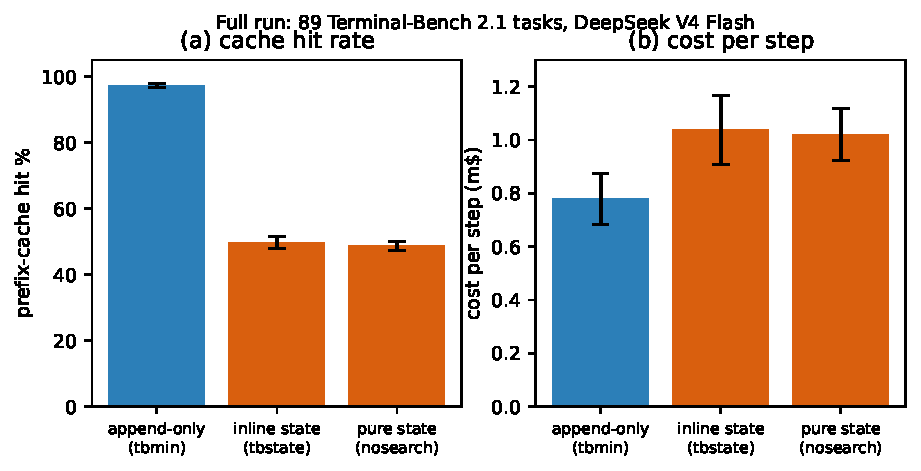
\includegraphics[width=0.8\textwidth]{figs/fig1_fullrun.pdf}
\caption{Cache hit rate (a) and cost per step (b). Compression buys fewer tokens
but a collapsed cache, and the cache loss dominates.}
\label{fig:full}
\end{figure}

\paragraph{The accuracy gap is a throughput confound, not reasoning.}
The full-run pass rate of the state arms looks slightly lower, but this is
explained entirely by timeouts, not by worse decisions. The state arm spends
8.6s of model time per step versus 5.8s for append-only, because it emits
$\sim$400 extra output tokens per step to rewrite the block and reasons over a
less cache-warm prompt. Over a 900s wall-clock budget, the slower arm hits more
timeouts (23--24 vs 16). On tasks where neither timed out, accuracy is identical.
Progressive disclosure (\texttt{search\_history}) added nothing: the inline and
nosearch arms are statistically indistinguishable.

\paragraph{Seed-variance check.} To confirm the accuracy neutrality is not an
artifact of single trials, we reran three arms (append-only, pure state, Tier~0)
on a 10-task subset with $k=3$ trials each. Mean per-task pass rates are
$76.7\pm24.0\%$, $70.0\pm24.7\%$ and $70.0\pm24.7\%$ respectively (95\% CI across
tasks): the intervals overlap almost completely, so the arms are accuracy-neutral
once run-to-run noise is accounted for. The apparent gaps trace to one or two
tasks whose three trials split (e.g.\ \texttt{db-wal-recovery} passes 1/3 vs
0/3), i.e.\ within-task seed variance exceeds the between-arm difference. Cost per
task preserves the ordering of Section~\ref{sec:fullrun}: append-only \$0.105,
pure state \$0.139 ($+32\%$), Tier~0 \$0.151 ($+44\%$).

\section{Result 2: a cost break-even law}
\label{sec:breakeven}
Let per step each arm consume $u$ uncached (miss) tokens, $h$ cached (hit)
tokens, and $o$ output tokens, priced $p_m, p_c, p_o$. Cost per step is
$C = u\,p_m + h\,p_c + o\,p_o$. Write the cache discount $r = p_c/p_m$ and the
output ratio $\rho = p_o/p_m$. Structured state (subscript $s$) beats
append-only (subscript $b$) when $C_s < C_b$, i.e.
\[
r \;>\; r^\star \;=\; \frac{(u_b - u_s) + \rho\,(o_b - o_s)}{h_s - h_b}.
\]
Since append-only has a far larger cached prefix ($h_b \gg h_s$) the denominator
is negative, and because state re-encodes more ($u_s > u_b$) and outputs more
($o_s > o_b$) the numerator is negative, so $r^\star > 0$: there is a genuine
threshold. Plugging in the across-task per-step means (append-only
$u_b{=}588, h_b{=}35990, o_b{=}687$; pure state
$u_s{=}4739, h_s{=}4548, o_s{=}1047$) with $\rho=2$ gives
\[
r^\star = \frac{(588-4739) + 2(687-1047)}{4548-35990}
        = \frac{-4871}{-31442} = 0.155 .
\]
At the price our run was billed, DeepSeek charged $r = 0.014/0.14 = 0.10 <
r^\star$, so append-only wins (Figure~\ref{fig:be}); a subsequent price cut took
the cache hit to $r=0.02$, only strengthening the result
(Section~\ref{sec:providers}). The law makes the dependence explicit: structured
state only pays off on a provider whose cache discount is \emph{weaker} than
about $6.5{:}1$. As the cache hit approaches free ($r\to0$), $r^\star$ stays
strictly positive, so \textbf{the cheaper the cache, the more decisively
append-only wins} --- the opposite of the token-count intuition.

\begin{figure}[h]\centering
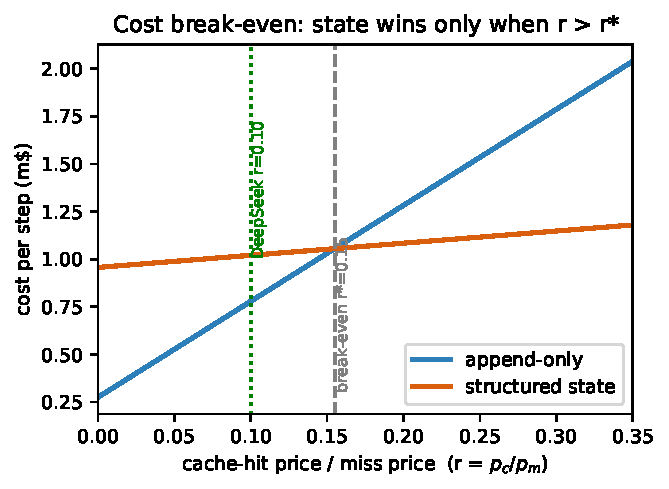
\includegraphics[width=0.5\textwidth]{figs/fig2_breakeven.pdf}
\caption{Cost per step vs.\ cache discount $r$. The arms cross at $r^\star=0.155$;
DeepSeek's $r=0.10$ sits on the append-only side.}
\label{fig:be}
\end{figure}

\subsection{Where today's providers sit}
\label{sec:providers}
Because $r^\star$ is a price threshold, the method could in principle win or lose
by choice of provider. We therefore surveyed real September 2026 price sheets
for the current workhorse model of each major provider, holding our measured
per-step token counts fixed and varying only price (Table~\ref{tab:prov},
Figure~\ref{fig:prov}). The finding is that the market has converged below the
threshold: every provider prices its cache hit at $r\le0.10$, so append-only wins
everywhere, by $1.37\times$ on the $r=0.10$ providers and by $2.6$--$3\times$ on
DeepSeek, whose post-cut cache hit ($r=0.02$) is the cheapest of all. The law
also says what \emph{would} flip the verdict --- a provider pricing its cache
above $r^\star\approx0.16$ --- but no current provider is there, and the recent
moves (DeepSeek's cut) push further in the opposite direction. The widely
repeated claim that compacting context ``saves money'' is thus false on every
provider we can bill today. (Token counts are model-specific; we fix our
DeepSeek-run trajectory and vary only price, isolating the price effect.)

\begin{table}[h]\centering
\begin{tabular}{lcccc}
\toprule
model (Sept 2026) & $r=p_c/p_m$ & append m\$/step & state m\$/step & winner\\
\midrule
DeepSeek V4-Flash (post-cut) & 0.020 & 0.375 & 0.969 & append ($2.58\times$)\\
DeepSeek V4-Pro 0813 & 0.008 & 0.984 & 2.989 & append ($3.04\times$)\\
OpenAI GPT-5.6 & 0.100 & 30.49 & 41.72 & append ($1.37\times$)\\
Gemini 3.8 Flash & 0.100 & 5.717 & 7.822 & append ($1.37\times$)\\
Claude Sonnet 5 & 0.100 & 22.87 & 31.29 & append ($1.37\times$)\\
\bottomrule
\end{tabular}
\caption{Same trajectory, real Sept-2026 price sheets. All providers sit below
$r^\star$, so append-only wins on every one. (Prices from public API pages;
$r^\star=0.155$--$0.189$ depending on each provider's output/input ratio.)}
\label{tab:prov}
\end{table}

\begin{figure}[h]\centering
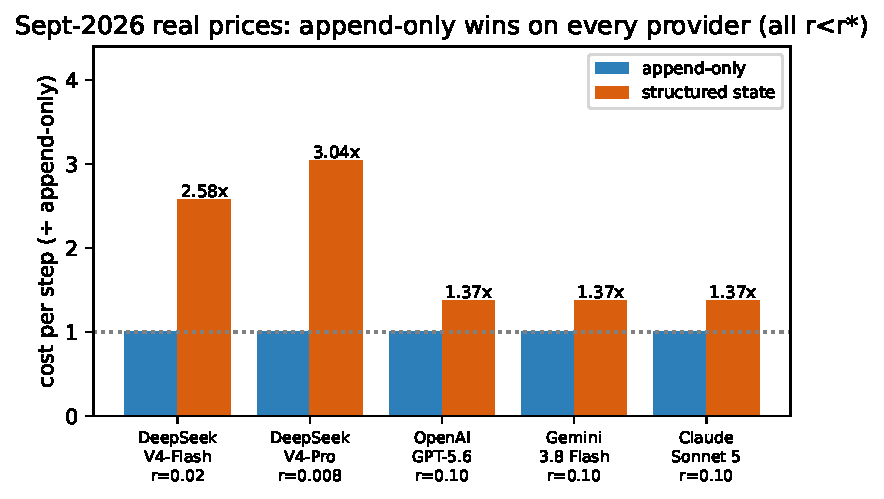
\includegraphics[width=0.65\textwidth]{figs/fig5_providers.pdf}
\caption{Per-step cost normalized to each provider's append-only cost. Structured
state is more expensive ($>1$) on every current provider; it would fall below 1
only for $r>r^\star$, which none reach.}
\label{fig:prov}
\end{figure}

\subsection{A second crossover: task length}
\label{sec:length}
The price threshold $r^\star$ assumes fixed per-step token counts, but those
counts grow as a task runs. Append-only's cached prefix lengthens every step, so
its per-step cost rises at $0.018$ m\$/step; structured state carries a bounded
block and rises at only $0.012$ m\$/step (Figure~\ref{fig:len}a). The lines cross
at a task length of $t^\star\approx68$ steps: beyond that horizon, append-only is
\emph{more} expensive per step even on DeepSeek's cheap cache, because a 10$\times$
discount on an ever-growing prefix still accumulates. A third (32.6\%) of our
tasks run past $t^\star$ (median length 52 steps, p90 109). Cumulatively append
still wins at observed lengths (Figure~\ref{fig:len}b; $0.77\times$ at step 60),
because its early steps were far cheaper and a long sustained per-step deficit is
needed to flip the running total --- but the trend is clear and sets where the
space axis (Section~\ref{sec:law}) begins to bite: not at the context-window
limit, but earlier, at the point where accumulated cheap-cache reads overtake a
compact rewrite.

\begin{figure}[h]\centering
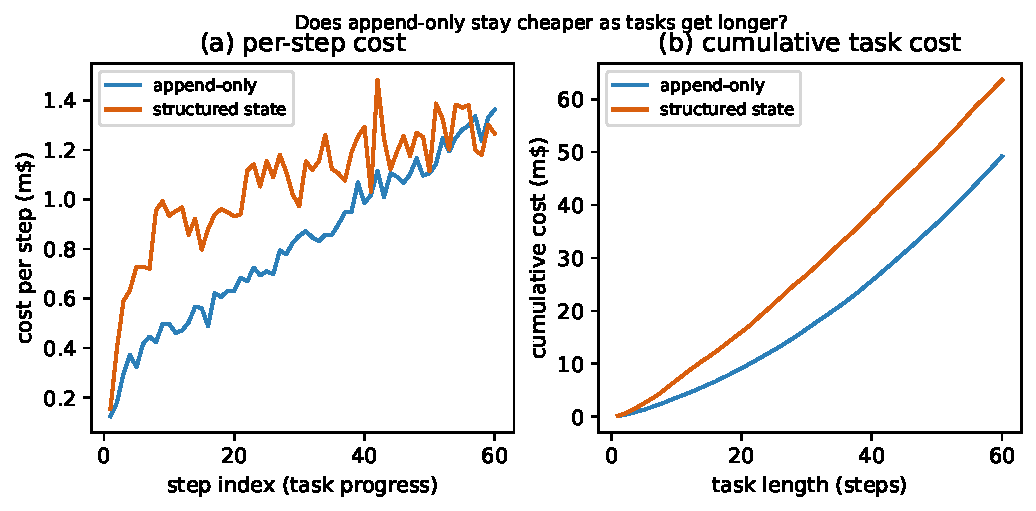
\includegraphics[width=0.85\textwidth]{figs/fig4_length.pdf}
\caption{(a) per-step cost vs task progress; append-only grows faster and crosses
structured state near step 68. (b) cumulative task cost; append still leads at
observed task lengths.}
\label{fig:len}
\end{figure}

The slopes above were billed at the price our run actually paid ($r=0.10$);
expressed in context length, the crossover $t^\star$ maps to a balance point
$H^\star$ --- the accumulated history at which append-only stops being the
cheaper per-step option. Holding the trajectory fixed and varying only price (as
in Section~\ref{sec:providers}), $H^\star$ depends sharply on $r$
(Table~\ref{tab:ctx}, Figure~\ref{fig:ctx}). At $r=0.10$ (OpenAI, Gemini,
Anthropic) the crossover survives at $H^\star\approx131$k tokens --- a fraction
of the window that ranges from 13\% (Gemini's 1M) to 65\% (Anthropic's 200k), so
the cost reason to compress can arrive before the window fills. But DeepSeek's
post-cut cache ($r=0.02$) is cheap enough that append-only's per-step cost slope
never overtakes structured state's: there is \emph{no} length crossover at all,
and append-only is cheaper at every context length up to the window limit. This
is the $r\to0$ limit made concrete --- as the cache approaches free, the
length-driven case for compression vanishes and only the hard window constraint
remains.

\begin{table}[h]\centering
\begin{tabular}{lcccc}
\toprule
model (Sept 2026) & $r$ & $H^\star$ (tokens) & window & $H^\star/$window\\
\midrule
DeepSeek V4-Flash (post-cut) & 0.020 & none (append always wins) & 128k & ---\\
OpenAI GPT-5.6 & 0.100 & 130{,}998 & 272k & 0.48\\
Gemini 3.8 Flash & 0.100 & 130{,}998 & 1000k & 0.13\\
Claude Sonnet 5 & 0.100 & 130{,}998 & 200k & 0.65\\
\bottomrule
\end{tabular}
\caption{Context-length balance point $H^\star$ at real prices. Append-only
prompt grows $\approx1284$ tokens/step; trajectory fixed, price varied.}
\label{tab:ctx}
\end{table}

\begin{figure}[h]\centering
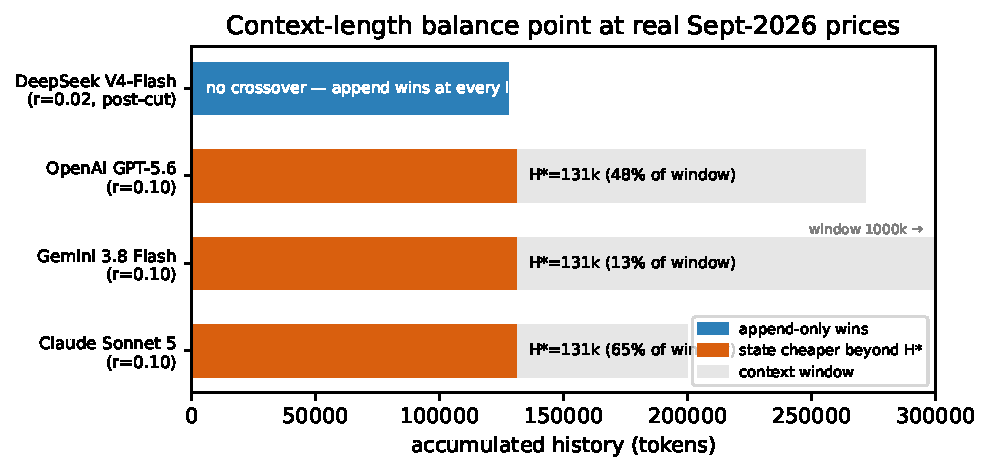
\includegraphics[width=0.72\textwidth]{figs/fig6_ctxbalance.pdf}
\caption{$H^\star$ against each model's window. At $r=0.10$ the crossover sits at
$\approx131$k tokens; DeepSeek's $r=0.02$ removes it, append-only winning at
every length.}
\label{fig:ctx}
\end{figure}

\section{Result 3: cache-aligned state (Tier~0) narrows but does not close}
\label{sec:tier0}
If the problem is that editing the middle invalidates the suffix, move the
mutable part to the \emph{end}. We built an append-only layout: a stable
preamble and immutable task first, then an append-only one-line action log, then
a small mutable ``current state'' tail. On a 20-task pilot this raised the hit
rate from 48\% to 58\% and cut cost per step 9\% versus inline state. But it
still lost to raw append-only (58\% vs 98\% hit; 0.882 vs 0.669 m\$/step),
because compression shrinks the \emph{cacheable} prefix about sixfold
(30{,}794$\to$5{,}423 cached tokens/step). You cannot get a large cache benefit
from a small cached region. Tier~0 confirms the mechanism: the penalty is the
lost cache mass, not merely edit position.

\section{Result 4: position-independent KV reuse (Tier~1) fails}
\label{sec:tier1}
The deeper fix would be a KV cache that reuses a span by \emph{content}
regardless of its position, so a rewritten-but-unchanged fact still hits. We
implemented this on an IBM vLLM fork (MiniPIC), which stores unrotated keys and
applies RoPE dynamically in the attention kernel, and hashes a span
independently of its predecessor. We replayed 268 real state prompts from our
Tier~0 run across three arms (append, span, span-reuse) on Qwen3-8B and on a
block-attention-finetuned model (Tulu3-Block-FT). Two findings (Figure~\ref{fig:t1}):
\begin{enumerate}[leftmargin=*,itemsep=1pt]
\item \textbf{No cost gain.} Block padding overhead erased the extra reuse:
span-reuse hit 74\% on Qwen3 and 73\% on Tulu3, both below plain append (77\% /
94\%).
\item \textbf{Accuracy collapse.} Block attention over many small state spans
agreed with full attention on only 7.7\% of greedy next tokens for Qwen3, and
35\% even for the model finetuned for block attention (whose finetuning targeted
a few large RAG documents, not many tiny agent-state spans).
\end{enumerate}
Escaping the cache's positional dependence at the serving layer is not free: the
model's learned distribution assumes the positions it was trained on.

\begin{figure}[h]\centering
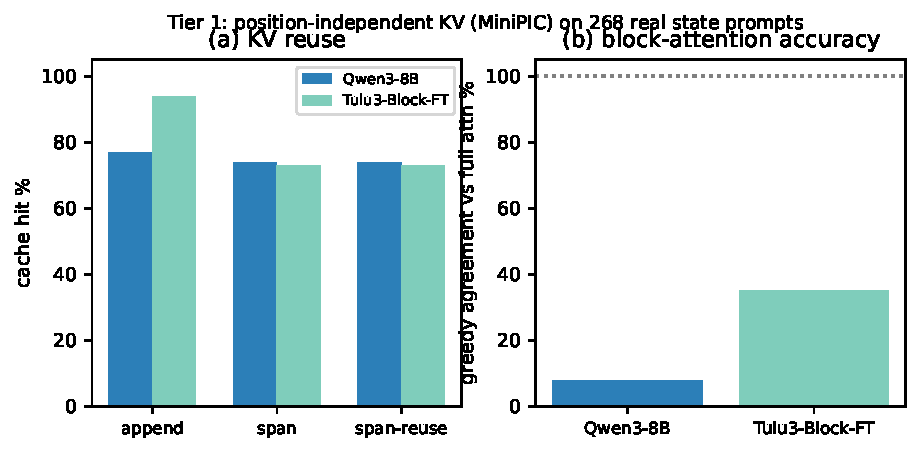
\includegraphics[width=0.8\textwidth]{figs/fig3_tier1.pdf}
\caption{Tier~1. (a) span reuse gives no hit-rate gain; (b) block attention
destroys agreement with full attention.}
\label{fig:t1}
\end{figure}

\section{Result 5: generality --- a second model family and a second benchmark}
\label{sec:general}

\subsection{Second model: Gemini 3.5 Flash, and the cache-reliability input}
\label{sec:gemini}
We reran append-only and pure structured state on a 10-task Terminal-Bench 2.1
subset with Gemini 3.5 Flash (list price \$1.50 / \$0.15 cached / \$9.00 per M;
nominal $r=0.10$, $\rho=6$, hence $r^\star=0.201$).\footnote{Gemini 3.8 Flash,
released 2 September 2026, did not report any implicit-cache hits in our tests
(four identical 12k-token prefixes, \texttt{cachedContentTokenCount} absent
every time), so its cache economics cannot be measured; 3.5 Flash is the newest
Gemini Flash whose implicit cache is observable.} Gemini's implicit cache is
\emph{best-effort}: the provider decides what stays warm. This turns out to
matter more than the price sheet.

\paragraph{Realized hit rate is far below nominal on short prompts.} Across 572
append-only steps the token-weighted realized hit rate is 89.4\%, versus
97--99\% on DeepSeek's deterministic prefix cache. The shortfall is concentrated:
prompts under 20k tokens hit only 48.6\% and \emph{49\% of those steps get zero
cache}; prompts above 20k hit 88--94\% with essentially no zero-hit steps
(Figure~\ref{fig:gem}b). Short tasks therefore run at nearly full price.

\paragraph{The law predicts a knife-edge, and that is what we observe.} Plugging
the \emph{realized} split into the law gives append-only an effective cache
discount $r_{\text{eff}} = (u\,p_m + h\,p_c)/((u{+}h)\,p_m) = 0.195$ --- almost
double the nominal $0.10$ and within $0.006$ of $r^\star=0.201$. The law thus
predicts a near-tie, and the paired results are exactly that: structured state
is cheaper on only 2 of 10 tasks; excluding one outlier, append-only is
$2.22\times$ cheaper (\$2.29 vs \$5.08); yet the aggregate is \$7.32 vs \$6.59
($0.90\times$, state cheaper), because a single task dominates
(Figure~\ref{fig:gem}a). That task (\texttt{db-wal-recovery}) is a runaway
trajectory: the append-only agent looped for 281 steps until the 900s timeout,
its prompt reaching 197k tokens and 21.5M cumulative prompt tokens (\$5.03, 69\%
of the arm's total), while the state arm stopped at 58 steps. With the realized
89.4\% hit, Gemini's length crossover falls to $H^\star\approx66$k tokens (from
131k at nominal price), and 197k is far past it --- the state win on that task
is precisely what Section~\ref{sec:length} predicts. Pass rates are noisy and
overlapping ($60\pm32\%$ vs $50\pm33\%$).

\paragraph{Cache reliability is a third input.} Two providers with the same
nominal $r=0.10$ land on opposite sides of the threshold once realized hit
rates are used: a deterministic prefix cache (DeepSeek, $r_{\text{eff}}\approx
r$) leaves append-only decisively cheaper; a best-effort implicit cache (Gemini,
$r_{\text{eff}}\approx 2r$) puts the verdict on the knife-edge and lets it flip
on long or runaway tasks. The provider comparison of Section~\ref{sec:providers}
must therefore be read with realized, not nominal, hit rates; and append-only's
cost on runaway loops grows roughly quadratically, which compression bounds.

\begin{figure}[h]\centering
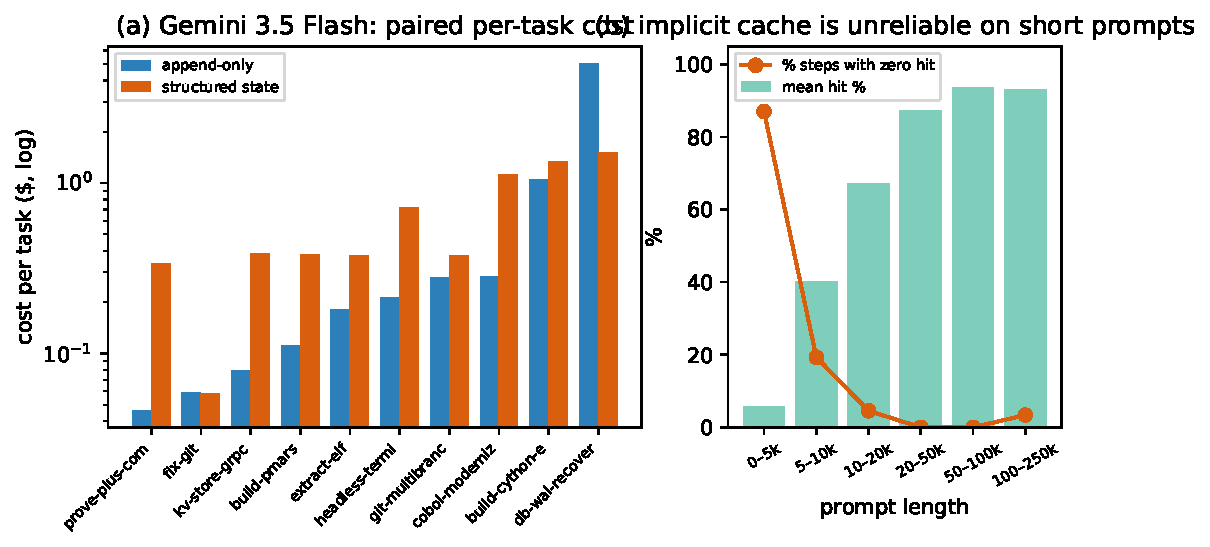
\includegraphics[width=0.95\textwidth]{figs/fig7_gemini.pdf}
\caption{Gemini 3.5 Flash. (a) Paired per-task cost (log scale): append-only
wins 8/10, but one runaway task flips the aggregate. (b) Realized implicit-cache
hit rate vs prompt length: unreliable below 20k tokens.}
\label{fig:gem}
\end{figure}

\subsection{Second benchmark: SWE-bench Verified}
\label{sec:swe}
To test a different task distribution --- repository-level bug fixing rather
than terminal tasks --- we ran append-only and pure structured state with
DeepSeek V4 Flash on a 22-task subset of SWE-bench Verified spanning 12
repositories (per-repository cap so Django does not dominate), $k=1$. The
result reproduces the main finding with no timeouts on either arm
(Table~\ref{tab:swe}, Figure~\ref{fig:swe}). Accuracy is identical: 21/22 in
both arms, failing the same task. Cache hit rate again collapses from 97.4\% to
49.9\%, and structured state costs $2.09\times$ more per task (\$0.089 vs
\$0.042; \$1.95 vs \$0.93 in total), being cheaper on only 5 of 22 tasks and
never by a meaningful margin. The realized discount is $r_{\text{eff}}=0.116$
against $r^\star=0.155$, so the law predicts append-only, as observed; unlike
Gemini, DeepSeek's deterministic prefix cache keeps $r_{\text{eff}}$ close to
nominal. Structured state also takes more steps (median 68 vs 61) and more model
time per step (3.6s vs 2.2s), the same throughput penalty seen in
Section~\ref{sec:fullrun}.

\begin{table}[h]\centering
\begin{tabular}{lccccc}
\toprule
arm & pass & cache hit \% & \$/task & out/task & model time/step\\
\midrule
append-only & 21/22 & $97.4\pm0.5$ & $0.042\pm0.015$ & 14{,}378 & 2.2s\\
pure state & 21/22 & $49.9\pm2.2$ & $0.089\pm0.044$ & 37{,}479 & 3.6s\\
\bottomrule
\end{tabular}
\caption{SWE-bench Verified, 22 tasks, DeepSeek V4 Flash. $\pm$ is a 95\% CI
across tasks.}
\label{tab:swe}
\end{table}

\begin{figure}[h]\centering
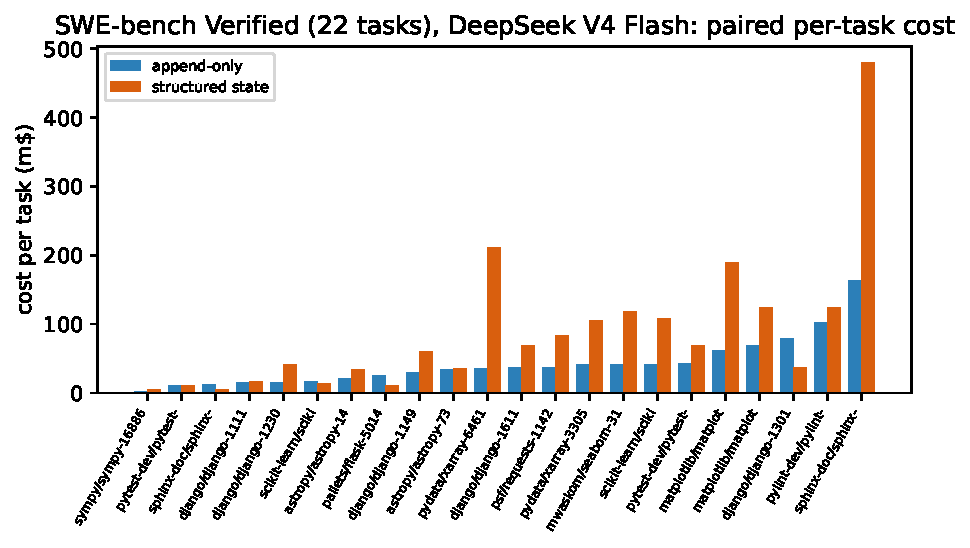
\includegraphics[width=0.8\textwidth]{figs/fig8_swe.pdf}
\caption{SWE-bench Verified: paired per-task cost. Structured state is cheaper
on 5 of 22 tasks and $2.09\times$ more expensive overall.}
\label{fig:swe}
\end{figure}

\section{A two-axis law for context management}
\label{sec:law}
The results resolve into one principle. A context-management scheme is evaluated
on two independent axes:
\begin{itemize}[leftmargin=*,itemsep=1pt]
\item \textbf{Price.} Under a prefix cache, seen tokens are nearly free, so the
billed quantity is uncached re-encodes plus output, not total tokens. On this
axis append-only is optimal whenever the history is a growing prefix, and any
rewrite is a strict loss (Sections~\ref{sec:fullrun}--\ref{sec:breakeven}).
\item \textbf{Space.} The context window is finite, and decode-time attention
cost grows with occupied length. On this axis, once history would overflow the
window (or the per-step attention cost becomes the bottleneck), compression is
\emph{necessary}, independent of price.
\end{itemize}
The two axes are not fully independent once history is allowed to grow. On the
price axis the winner is set by the provider's cache discount relative to
$r^\star$ (Section~\ref{sec:providers}); on the space axis, append-only's
per-step cost climbs with accumulated history and crosses compression at a task
length $t^\star$ (Section~\ref{sec:length}) that arrives \emph{before} the
context-window limit. So compression is justified whenever any of three
conditions holds: the provider's cache discount is weak ($r>r^\star$), where
$r$ must be the \emph{realized} discount $r_{\text{eff}}$ --- a best-effort
cache that misses 10\% of tokens roughly doubles it (Section~\ref{sec:gemini});
the task horizon is long ($t>t^\star$); or the history overflows the window. As of
September 2026 the first condition is met by no major provider, and DeepSeek's
price cut removes the second on its own models, so for most real deployments only
the hard window constraint remains --- which is the regime today's agentic
benchmarks inhabit and the reason the token-savings intuition has gone
unchallenged. This reframes SKILL.state and its relatives not as a universal
cost optimization but as a mechanism whose payoff is decided by two measurable
thresholds and one hard constraint.

\section{Related work}
SKILL.state and structured-memory agents motivate this study; our finding is that
their token savings do not translate to cost under prefix caching. Prefix/KV
caching (vLLM PagedAttention, SGLang RadixAttention) is the economic substrate we
analyze. CacheBlend and LMCache attempt cross-request, non-prefix KV reuse; at
the time of writing their V1 non-prefix path is non-functional, so we used the
MiniPIC fork instead and reached a negative result consistent with the
positional-dependence argument. Context compaction and recurrent-summary methods
live on the space axis of our law.

\section{Limitations}
\label{sec:limits}
Our main run is one benchmark and one model family; the generality check adds a
second model on a 10-task subset and a second benchmark on a 22-task subset,
both with $k=1$, so those estimates are coarse. The break-even law is general but
its value $r^\star$ is workload dependent, and --- as Gemini shows --- its inputs
must be realized, not nominal, cache splits. Terminal-Bench tasks mostly fit the context window, which is exactly
the regime where our law predicts append-only wins; we did not measure a
long-horizon regime that overflows the window, where compression should become
necessary. Pass-rate error bars are wide ($\pm24\%$ on the $k=3$ seed-variance
subset), so we lean on cost, which is far less variable, for the quantitative
claims. The Tier~1 accuracy failure might be narrowed by a model
finetuned specifically for many-small-span block attention, which we did not train.

\section{Conclusion}
Replacing agent history with a compact structured state trades cheap cached
tokens for expensive re-encodes and extra output; whether that trade pays off is
not a matter of token count but of two measurable thresholds. On the price axis
it wins only when the provider's cache discount is weak ($r>r^\star\approx0.16$),
and no major provider prices its cache there today --- all sit at $r\le0.10$,
DeepSeek at $0.02$ after a cut. On the length axis it wins only past a context
length $H^\star$ that, at $r=0.10$, is $\approx131$k tokens and, on post-cut
DeepSeek, does not exist. It never improves accuracy on our benchmark, and
escaping the cache's positional dependence at the serving layer (Tier~1) costs
accuracy outright. The practical rule for today's providers: unless your history
overflows the context window, append only; structured state is a window-fit
mechanism, not a cost optimization, and would become one only if a provider
priced its cache above $r^\star$.
\end{document}
